
\section{Introduction to Programming}

\begin{frame}{Programming (1)}
\begin{itemize}
\item Executable programs are containing only \textbf{zeros and ones}, because
that is the only language that computer understands
\item Programmers write the programs in human readable
languages, called \textbf{programming languages}
\item Program written in programming language is called a \textbf{source code}
\end{itemize}
\end{frame}

\begin{frame}{Programming (2)}
\begin{itemize}
  \item Usually for writing source code programmers use \textbf{development
  environments}
  \item The code is written in text editor
  \item Then the code is (\textbf{compiled})
  \item At the end we have \textbf{executable} i.e. program written in machine
  language (the language of the computer)
\end{itemize}
\end{frame}

% Define block styles
\tikzstyle{block} = [rectangle, draw, fill=blue!20,
text width=5em, text centered, rounded corners, minimum height=4em]
\tikzstyle{line} = [draw, -latex']

\begin{frame}[fragile,shrink=20]{Compiling and executing process }

\begin{center}
Phase 1 - compiling the source code
\begin{tikzpicture}[node distance = 3cm, auto]
    % Place nodes
    \node [block] (compiler) {Compiler};
    \node [block, below of=compiler, node distance=2cm] (source) {Source code}; 
    \node [block, right of=compiler] (computer) {Computer};
    \node [block, right of=computer] (executable) {Executable (in memory)};
    % Draw edges
    \path [line] (compiler) -> node {} (computer);
    \path [line] (source) -| node {} (computer);
    \path [line] (computer) -> node {} (executable);
\end{tikzpicture}
\end{center}
\begin{center}
Phase 2 - execution
\begin{tikzpicture}[node distance = 3cm, auto]
    % Place nodes
    \node [block] (program) {Executable (in memory)};
    \node [block, below of=program] (data) {Input data};
    \node [block, right of=program] (computer) {Computer};
    \node [block, text width=3cm, right of=computer] (executable) {Execution
    result};
    % Draw edges
    \path [line] (program) -> node {} (computer);
    \path [line] (data) -| node {} (computer);
    \path [line] (computer) -> node {} (executable);
\end{tikzpicture}
\end{center}
\end{frame}


\begin{frame}{Introduction to C programming language}
\begin{itemize}
\item Developed in Bell laboratories in period from 1969 to 1973 by Dennis
Ritchie
\item One of the most used general purpose programming languages of all time
\item Has big influence in origins and development of many other programming
languages
    \begin{itemize}
    \item C++
    \item Objective C
    \item PHP
    \item Java
    \end{itemize}
\end{itemize}
\end{frame}

\begin{frame}[fragile]{C Syntax}

  \begin{block}{Allowed characters in C:}
  \begin{verbatim}
    a-z, A-Z, 0-9 and ~!@#$%^&*()-+={}[]:;'"<>?/._  
  \end{verbatim}
  \end{block}

    \begin{alertblock}{Attention!}
    Compiler is case sensitive (makes difference between uppercase and lowercase)!
    \end{alertblock}

    All characters in C are forming words that can be:
    \begin{enumerate}
    \item Keywords
    \item Numerical and symbolic constants
    \item Identifiers
    \item Strings (char arrays)
    \item Operators
    \end{enumerate}

\end{frame}

\begin{frame}{C Syntax}

    \begin{block}{Set of keywords (32)}

    \begin{tabular}{c c c c}
        \texttt{auto} & \texttt{double} & \texttt{int} & \texttt{struct} \\
        \texttt{break} & \texttt{else} & \texttt{long} & \texttt{switch} \\
        \texttt{case} & \texttt{enum} & \texttt{register} & \texttt{typedef} \\
        \texttt{char} & \texttt{extern} & \texttt{return} & \texttt{union} \\
        \texttt{const} & \texttt{float} & \texttt{short} & \texttt{unsigned} \\
        \texttt{continue} & \texttt{for} & \texttt{signed} & \texttt{void} \\
        \texttt{default} & \texttt{goto} & \texttt{sizeof} & \texttt{volatile} \\
        \texttt{go} & \texttt{if} & \texttt{static} & \texttt{while}
    \end{tabular}
    \end{block}
\end{frame}

\begin{frame}[fragile]{Simple C program structure}

    All the source code written in C is organized in \textbf{functions}
    \linebreak
    
    \begin{columns}[t]
        \column{.5\textwidth}
            \begin{block}{Program in C}
                \begin{lstlisting}
                int main() {
                    variable_declaration;
                    expressions;                    
                }
                \end{lstlisting}
            \end{block}
        \column{.5\textwidth}
            \begin{block}{Program in Pascal}
                \begin{lstlisting}
                Program program_name;
                var variable_declaration;
                begin
                    expressions;;
                end.
                \end{lstlisting}
            \end{block}
    \end{columns}

\end{frame}

\begin{frame}[shrink=10]{C Functions}
    \hfill
    \begin{block}{\texttt{main}}
         C main function
    \end{block}
    
    \begin{block}{\texttt{()}}
         In parentheses we put the input arguments
    \end{block}
    
    \begin{block}{\texttt{int}}
         Data type of the result it's before the function name
    \end{block}
    
    \begin{block}{\texttt{\{\}}}
         The function body starts with \{, and ends with \}
    \end{block}

    \begin{block}{\texttt{;}}
    All declarations and expressions are separated with \texttt{;}
    \end{block}

\end{frame}

\begin{frame}[fragile]{Comments usage}
    \begin{itemize}
        \item Comments are used for extra explanation or documenting the source code
        \item C supports two types of comments
        \begin{enumerate}
            \item one line comments
            \item multiple line comments
        \end{enumerate} 
        
    \end{itemize}
        
    \begin{columns}[t]
        \column{.5\textwidth}
            \begin{block}{1. One line comments}
                \begin{verbatim}
                // one line comment ;)
                \end{verbatim}
            \end{block}
        \column{.5\textwidth}
            \begin{block}{2. Multiple line comment}
                \begin{verbatim}
                /* Comment
                   in multiple lines */
                \end{verbatim}
            \end{block}
    \end{columns}       

\end{frame}

\begin{frame}[fragile]{Examples}
    \begin{exampleblock}{Example 1}
        \begin{lstlisting}
            #include <stdio.h>
            // main function
            int main() {
                /* function for print on standard output (screen) */
                printf("Welcome to FINKI!\n");
                return 0;
            }
        \end{lstlisting}
    \end{exampleblock}
\end{frame}

\begin{frame}{C program structure (extended)}
    \begin{columns}
        \column{.2\textwidth}
        \textbf{INCLUDE} section
        \column{.8\textwidth} contains \texttt{\#include} expressions for
        including external libraries, for using externally declared functions
    \end{columns}
    \hfill
    \linebreak
    \begin{columns}
        \column{.2\textwidth}
        \textbf{DEFINE} section
        \column{.8\textwidth} contains \texttt{\#define} expressions for constants and
        data type declaration
    \end{columns}   
    \hfill
    \linebreak
    \begin{columns}
        \column{.2\textwidth}
        ...
        \column{.8\textwidth} defining global variables and functions
    \end{columns}
    \hfill
    \linebreak
    \begin{columns}
        \column{.2\textwidth}
        \texttt{int main()}
        \column{.8\textwidth} main function
    \end{columns}
\end{frame}

\begin{frame}{Preprocessor}
\begin{itemize}
    \item In C compiling is done by:
    \begin{itemize}
        \item preprocessor
        \item compiler
    \end{itemize}
    \item The preprocessor is used with directives
    \begin{itemize}
        \item Each directive starts with \texttt{\#}
    \end{itemize}
\end{itemize}
\end{frame}

\begin{frame}{Header files}
\begin{itemize}
    \item One usage of preprocessor directive is including the ``header files''
    \begin{itemize}
        \item Used for declaration of functions and variables in some predefined
        library
        \item In order to use the external functions and variables users include the
        ``header file''
    \end{itemize}
    \item The inclusion is done with the preprocessor directive 
    \texttt{\#include}
    \begin{itemize}
        \item Statement \texttt{\#include} causes inclusion a copy of the given file
        in the place where the statement is written
    \end{itemize}
\end{itemize}
\end{frame}

\begin{frame}[fragile]{\texttt{include} variations}
\begin{itemize}
    \item There are two types of this directive:
    \begin{itemize}
        \item file that is included can be written in double quotes (""),
        \item or in angle brackets (<>)
    \end{itemize}
    \begin{exampleblock}{Example}
        \begin{verbatim}
        #include <filename.h>
        #include "filename.h"
        \end{verbatim}
    \end{exampleblock}
    \item The difference is in the location in which the preprocessor
    searches the file that should be included
    \begin{itemize}
        \item In angle brackets (files from the standard library are used)
        \item With double quotes (the preprocessor first tries to find
        the file in the same directory with the C file that should be
        compiled)
    \end{itemize}
\end{itemize}

\end{frame}

\begin{frame}{Variables}
\begin{itemize}
\item Variables are symbolic names for places in memory where the
computer keeps values
\item Before usage all variables must be \emph{declared}
\item With each new assignment of value, the old value is discarded
\end{itemize}

Types of variable declaration:
\linebreak
\begin{columns}
        \column{.32\textwidth} \fbox{Variable type}
        \column{.32\textwidth} \fbox{Variable name}
        \column{.05\textwidth} \fbox{ = }
        \column{.26\textwidth} \fbox{Initial value}
        \column{.05\textwidth} \fbox{ ; }
\end{columns}   

\end{frame}

\begin{frame}{Data types}
\Large{Data types in C}
\linebreak
\linebreak
\begin{tabular}{c|c|c}
\textbf{Numbers} & \textbf{Letters} & \textbf{Decimal}\\
\hline
\texttt{int} & \texttt{char} & \texttt{float} \\
\hline
\texttt{short} & & \texttt{double} \\
\hline
\texttt{long} & &
\end{tabular}
\end{frame}

\begin{frame}{Defining variable names}
\begin{itemize}
\item In naming variables allowed are:
\begin{itemize}
\item lowercase letters from a to z;
\item uppercase letters from A to Z;
\item digits from 0 to 9 (can't start with digit);
\item underscore \_ which is recognized as a letter (not recommended to start
with \_);
\end{itemize}
\end{itemize}
\begin{alertblock}{Be carefull!}
\begin{itemize}
\item mostly names length is up to 32 characters
\item С is case sensitive!
\end{itemize}
\end{alertblock}
\end{frame}

\begin{frame}[fragile]{Examples}
    \begin{exampleblock}{Example 2}
        \begin{lstlisting}
            #include <stdio.h>

            int main() {
                int a, b, c;
                a = 5;
                b = 10;
                c = a + b;
                return 0;
            }
        \end{lstlisting}
    \end{exampleblock}
\end{frame}

\begin{frame}{Constants}
\begin{itemize}
\item Constants are used for values that are unchanged during the program
execution
\item Each constant is from some data type
\item C has several constant types:
\begin{itemize}
\item decimal: \texttt{1, -23, 15}
\item octal: \texttt{015, 035, 0205}
\item hexadecimal: \texttt{0x25, 0xA4C}
\item real: \texttt{3.5F, -2.845F, 1.34e-9}
\item literals: \texttt{'a', '\_', 'e'}
\item strings: \texttt{" ", "Koncepti za razvoj na softver"}
\end{itemize}
\end{itemize}
\end{frame}

\begin{frame}{Determining constant type}
\begin{itemize}
\item Determining the type of varialbes is simple (can be seen from the
declaration)
\item Constants aren't declared, so their type is determined by the
way they are written:
\begin{itemize}
\item Numbers that contain "." or "е" are
{\color{blue}\texttt{double}}:
\texttt{3.5, 1е-7, -1.29е15}
\item Instead of using \texttt{double}, to use {\color{blue}{\texttt{float}}}
constants "F" is added at the end: \texttt{3.5F, 1e-7F}
\item For {\color{blue}\texttt{long double}} constants "L" is added:
\texttt{1.29е15L, 1e-7L}
\item Numbers without ".", "е" or "F" are {\color{blue}\texttt{int}}:
\texttt{1000, -35}
\item For {\color{blue}\texttt{long int}} constants "L" is added:
\texttt{9000000L}
\end{itemize}
\end{itemize}
\end{frame}

\begin{frame}[fragile]{Named constants (1)}
\Large{Named constants are created by using the keyworkd \texttt{const}}
\begin{exampleblock}{Example 3}
        \begin{lstlisting}
            #include <stdio.h>

            int main() {
                const long double pi = 3.141592653590L;
                const int days_in_week = 7;
                const sunday = 0; /* by default int */
                days_of_week = 1; /* error */
            }
        \end{lstlisting}
    \end{exampleblock}
\end{frame}

\begin{frame}[fragile]{Named constants (2)}
Named constants can be created with the preprocessor, and usually
uppercase letters are used
    \begin{exampleblock}{Example 3}
        \begin{lstlisting}
            #include <stdio.h>
            #define PI 3.141592653590L
            #define DAYS_IN_WEEK 7
            #define SUNDAY 7        
            int main() {
                long double pi = PI;
                int day = SUNDAY;
            }
        \end{lstlisting}
    \end{exampleblock}
\end{frame}

\begin{frame}{Operators}
\begin{itemize}
\item Operators are used in builing expressions, and operations are
evaluated from right to left by applying the operator priority rules
\item There are three types of operators
\begin{itemize}
\item Arithmetic operators
\item Relational operators
\item Logical operators
\end{itemize}
\end{itemize}
\end{frame}

\begin{frame}{Arithmetic operators}
Usen on numbers (integers or reals)
\linebreak
\begin{center}
\begin{tabular}{c|c}
\textbf{Operator} & \textbf{Operation}\\
\hline
\texttt{+} & Addition \\
\texttt{-} & Substruction \\
\texttt{*} & Multiplication \\
\texttt{/} & Division \\
\texttt{\%} & Division by modulo
\end{tabular}
\end{center}
\end{frame}

\begin{frame}{Relational operators}
Applyed on any comparable data types, and the result is 0 (false) or 1 (true).
\begin{center}
\begin{tabular}{c|c}
\textbf{Operator} & \textbf{Meaning}\\
\hline
\texttt{<} & Less than \\
\texttt{<=} & Less than or equal \\
\texttt{>} & Greater than \\
\texttt{>=} & Greater than or equal \\
\texttt{==} & equal \\
\texttt{!=} & not equal
\end{tabular}
\end{center}
\end{frame}

\begin{frame}{Logical operators}
Used mostly in combination with relational operators in forming complicated
logical expressions, which again results in 0 or 1
\linebreak
\begin{center}
\begin{tabular}{c|c}
\textbf{Operator} & \textbf{Operation}\\
\hline
\texttt{\&\&} & Logical AND \\
\texttt{||} & Logical OR \\
\texttt{!} & Negation
\end{tabular}
\end{center}
\end{frame}

\begin{frame}[fragile]{Additional operators}
\begin{itemize}
\item Assignment operator =
\item Increment and decrement operators
\begin{verbatim}
++, --
\end{verbatim}
\item Unary usage of operators + and –
  \begin{verbatim}
    X = + Y;
    X = - Y;
  \end{verbatim}
\item Double operators
\begin{itemize}
\item Combination of assignment operator and other operator
\begin{verbatim}
(+=, -=, *=, /=, %=)
\end{verbatim}
\end{itemize}
\end{itemize}
\end{frame}

\begin{frame}[fragile]{Assignment operator =}
\begin{itemize}
\item All expressions have values, even those containing =
\item Value of such expression is the value of the expression of the
right side
\item Because of that, this assignment is possible:
\end{itemize}
\begin{verbatim}
    x = (y = 10) * (z = 5);
    x = y = z = 20;
\end{verbatim}
\end{frame} 

\begin{frame}[fragile,shrink=5]{Double operators}
\begin{block}{Operator +=}
\begin{verbatim}
a += 5; // a = a + 5;
a += b * c; // a = a + b * c;
\end{verbatim}
\end{block}
\begin{block}{Operator -=}
\begin{verbatim}
a -= 3; // a = a – 3;
\end{verbatim}
\end{block}
\begin{block}{Operator *=}
\begin{verbatim}
a *= 3; // a = a * 3;
\end{verbatim}
\end{block}
\begin{block}{Operator /=}
\begin{verbatim}
a /= 3; // a = a / 3;
\end{verbatim}
\end{block}
\begin{block}{Operator \%=}
\begin{verbatim}
a %= 3; // a = a % 3;
\end{verbatim}
\end{block}
\end{frame} 

\begin{frame}[fragile]{Using variables and operators}
    \begin{exampleblock}{Example 4}
        \begin{lstlisting}
            #include <stdio.h>  
            int main() {
                int a;
                float p;
                p = 1.0 / 2.0; /* p = 0.5 */
                a = 5 / 2;     /* a = 2   */
                p = 1 / 2 + 1 / 8; /* p = 0; */
                p = 3.5 / 2.8; /* p = 1.25 */
                a = p; /* a = 1 */
                a = a + 1; /* a = 2; */
                return 0;       
            }
        \end{lstlisting}
    \end{exampleblock}
\end{frame}

\begin{frame}[fragile]{Printing to the standard output}
\begin{itemize}
\item In C doesn't exist printing command
\item Already defined function from the input/output library \texttt{stdio.h} is
used (\textbf{st}andar\textbf{d} \textbf{i}nput/\textbf{o}utput)
\large{\texttt{\#include <stdio.h>}}
\item The function used is:
\end{itemize}
\begin{verbatim}
int printf(control_array, list_of_arguments)
\end{verbatim}
\begin{itemize}
\item The control array contains any string, formating and printing arguments
with leading \% or special characters with leading \textbackslash.
\item Characters for formating are determined from the data type that
should be printed.
\end{itemize}
\end{frame}

\begin{frame}{Formatting characters}
\begin{scriptsize}
\begin{tabular}{|c|l|}
\hline \textbf{Character} & \textbf{Explanation} \\ 
\hline \texttt{\%d} & integers \\ 
\hline \texttt{\%i} & integers \\ 
\hline \texttt{\%c} & single character \\ 
\hline \texttt{\%s} & char arrays \\ 
\hline \texttt{\%e} & real number in technical foramat (е) \\
\hline \texttt{\%E} & real number in technical foramat (Е) \\ 
\hline \texttt{\%d} & real number in decimal foramat \\ 
\hline \texttt{\%f} & real number in shorter from the foramats \%е and \%f \\ 
\hline \texttt{\%g} & real number in shorter from the foramats \%Е and \%f \\  
\hline \texttt{\%u} & unsigned integer \\ 
\hline \texttt{\%o} & unsigned integer in octal \\ 
\hline \texttt{\%x} & unsigned hexadecimal integer \\
\hline \texttt{\%X} & unsigned hexadecimal integer \\ 
\hline \texttt{\%p} & pointer \\ 
\hline \texttt{\%n} & number of printed characters \\
\hline \texttt{\%\%} & printing the character \% \\ 
\hline 
\end{tabular} 
\end{scriptsize}
\end{frame}

\begin{frame}[fragile]{Function \texttt{printf} usage}
    \begin{exampleblock}{Example 5}
        \begin{lstlisting}
        #include <stdio.h>
        int main() {
           printf(" length is %d letters.\n", printf("Makedonija"));
           return 0;
        }
        \end{lstlisting}
    \end{exampleblock}
\end{frame}

\begin{frame}[fragile]{Problem 1}
    Write a program that will compute the value of the mathematical expression:
    $ x = \frac{3}{2} + (5 - \frac{46 * 5}{12})$
    \begin{exampleblock}{Solution}
    \lstinputlisting{src/av1/p1.c}
    \end{exampleblock}
\end{frame}

\begin{frame}[fragile]{Problem 2}
Write a program that for a given value of $ x $ (with the declaration
assignment) will compute and print on standard output $ x^2 $.
    \begin{exampleblock}{Solution}
    \lstinputlisting{src/av1/p2.c}
    \end{exampleblock}
\end{frame}

\begin{frame}[fragile]{Problem 3}
Write a program that for a given sides of one triangle, it will print the
perimeter and area of the square (values are \texttt{a=5, b=7.5,
c=10.2}).
    \begin{exampleblock}{Solution}
    \lstinputlisting{src/av1/p3.c}        
    \end{exampleblock}
\end{frame}

\begin{frame}[fragile]{Problem 4}
Write a program for computing the arithmetic mean of the numbers 3, 5 and 12.
    \begin{exampleblock}{Solution}
    \lstinputlisting{src/av1/p4.c}
    \end{exampleblock}
\end{frame}

\begin{frame}[fragile]{Problem 5}
Write a program that will print the remainder from the division of number 19
with 2, 3, 5 and 8.
    \begin{exampleblock}{Solution}
    \lstinputlisting{src/av1/p5.c}        
    \end{exampleblock}
\end{frame}

\section{Development environments (IDE)}

\begin{frame}{Integrated development environments elements}
Integrated development environment is mix of multiple programs, that are
combined in order to simplify the development process
\begin{itemize}
  \item text editor
  \item compiler
  \item debugger
  \item external library integration
  \item linker
\end{itemize}
\end{frame}

\begin{frame}{Text editor}
\begin{itemize}
  \item Program for inserting and editing the text of the source code
  \item Enables saving and loading already written source code files
  for editing
  \item Syntax highlighting
\end{itemize}
\end{frame}

\begin{frame}{Compiler}
\begin{itemize}
  \item Transforms (translates) the source code from the programming language
  (high level) to machine language
  \item Two types of code translators:
  \textbf{interpreters} and \textbf{compilers}
  \item Interpreter is a translator of source code which \emph{translates each
  command separately}, checks for errors and executes, and goes to the next
  command.
  \item Compiler is a translator which is \emph{processing the whole
  program}, checks for errors, and creates the executable program.
  \begin{itemize}
  \item The resulted executable can be executed
  \end{itemize}
\end{itemize}
\end{frame}

\begin{frame}{Debugger}
\begin{itemize}
  \item Compilers and interpreters are detecting the (syntax) errors of the
  source code as a result from incorrect usage of the programming language
  \item Other type of errors are logical errors
  \begin{itemize}
  \item The program doesn't execute as intended
  \item Very difficult to discover
  \end{itemize}
  \item Debugger is a program that helps discovering logical errors
  \begin{itemize}
  \item Enables execution step by step
  \end{itemize}
\end{itemize}
\end{frame}

\begin{frame}{Integration with external libraries}
\begin{itemize}
  \item Integration and usage of already created and correct modules,
  also called functions
  \item This type of organization has many advantages
  \item Reuse of standard functions
  \item Example libraries
  \begin{itemize}
    \item Standard input/output
    \item Mathematical operations 
  \end{itemize}
\end{itemize}
\end{frame}

\begin{frame}{Linker}
\begin{itemize}
  \item Sometimes the program is to large to be written in one file
  \begin{itemize}
    \item different parts can be written by different programmers
    \item some parts from one program can be used in some other program
    \item Separately compiled parts must be united in on full executable with
    the help of the \textbf{linker}
    \item Another role is to ``link'' standard functions with the executable
  \end{itemize}
\end{itemize}

\end{frame}

\begin{frame}{Integrated Development Environment - IDE}
\begin{itemize}
  \item All these elements of the development environment are integrated in IDE
  \item Code::Blocks is an example of IDE that can be used in this course
\end{itemize}
\begin{center}
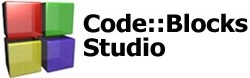
\includegraphics[scale=0.5]{images/cb_logo}
\end{center}
\end{frame}

\section{Code::Blocks - installation}
\begin{frame}{Code::Blocks - installation}
\begin{itemize}
  \item How to find and install Code::Blocks
  \item Code::Blocks is \textbf{free software} and can be find \linebreak
  \href{http://www.codeblocks.org/downloads}{http://www.codeblocks.org/downloads}
  \item In the central part of the page, there are three links:
  \textbf{Download the binary release}, Download the source code and Retrieve
  source code from SVN
  \item The first link is recommended for most simple installation
  - \textbf{Download the binary release},
\end{itemize}
\end{frame}

\begin{frame}{Code::Blocks – installation (2)}
\begin{itemize}
  \item For begginers is recommended the version that includes \textbf{MinGW} setup
    \begin{itemize}
  \item at the moment that is the link \textbf{codeblocks-10.05mingw-setup.exe}
  which supports all \textbf{Windows} operating systems
  \item By clicking the source Sourceforge.net opens up a new page, and after 5
  seconds the page will show you option to save the file in some location
  \item After saving the file follow the installation instructions
    \end{itemize}
\end{itemize}
\end{frame}

\begin{frame}{Code::Blocks – main window}
\begin{center}
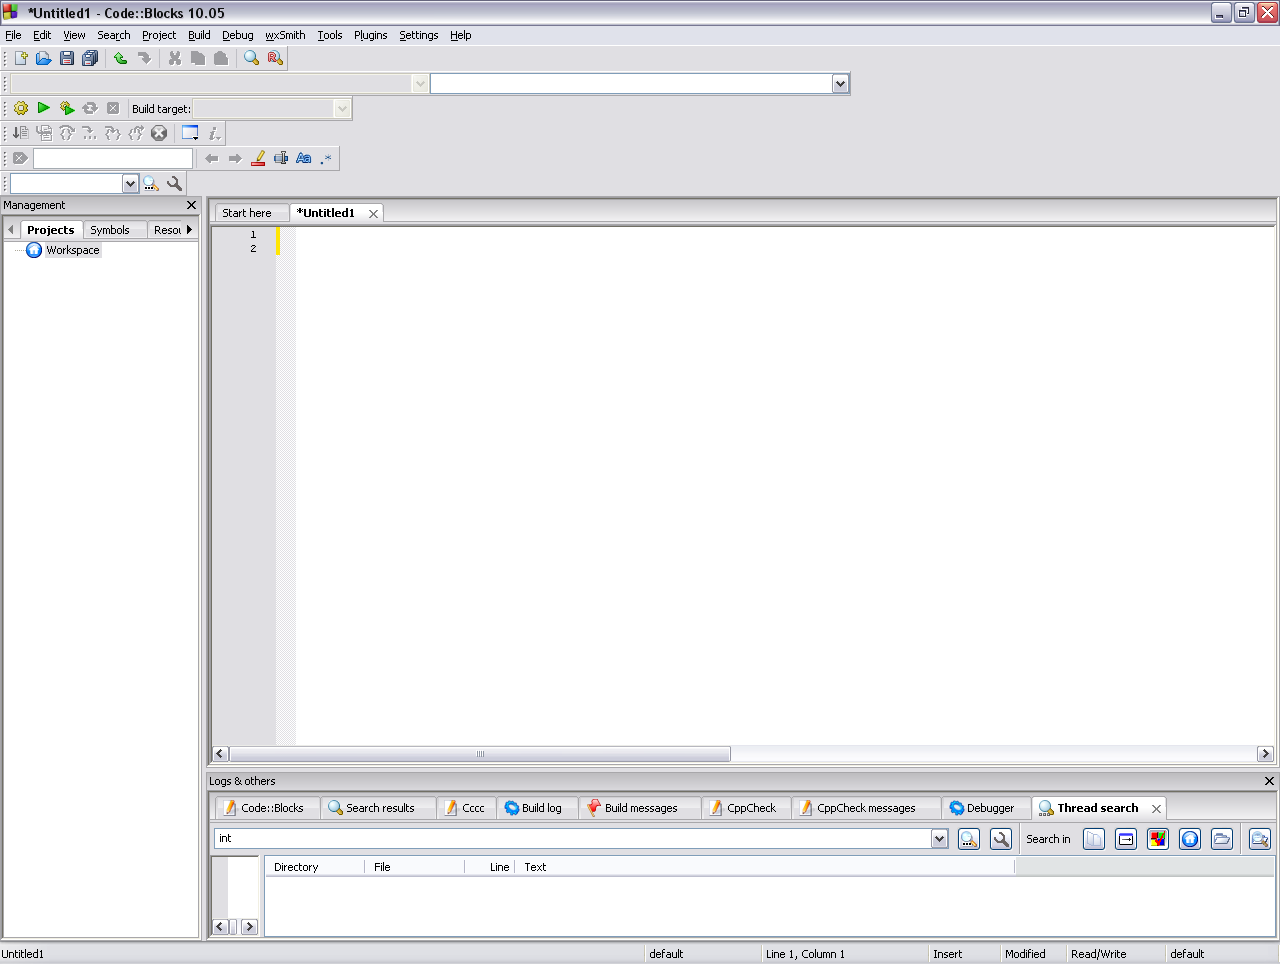
\includegraphics[scale=0.26]{images/cb_main}
\end{center}
\end{frame}

\begin{frame}{Elements of the main window}
\begin{itemize}
  \item Menu strip
    \begin{itemize}
      \item Menu strip is in to top left corner of the window, right
      bellow the title
      \item There can be found menues File, Edit,
      View, Search, Project, Build, Debug, wxSmith, Tools, Plugins, Settings, Help
    \end{itemize}
    \item Toolstrip
    \begin{itemize}
      \item Toolstrip (buttons for starting most often used commands) are just
      bellow the menu strip
    \end{itemize}
    \item Workspace
    \begin{itemize}
      \item Text editor
      \item Info window for logs \& others
      \item Window for management
    \end{itemize}   
\end{itemize}
\end{frame}

\begin{frame}{Programming in C with Code::Blocks}{Creating project}
\begin{enumerate}
  \item Start CodeBlocks
  \item File -> New -> Project -> Empty Project -> Go 
\end{enumerate}
\begin{center}
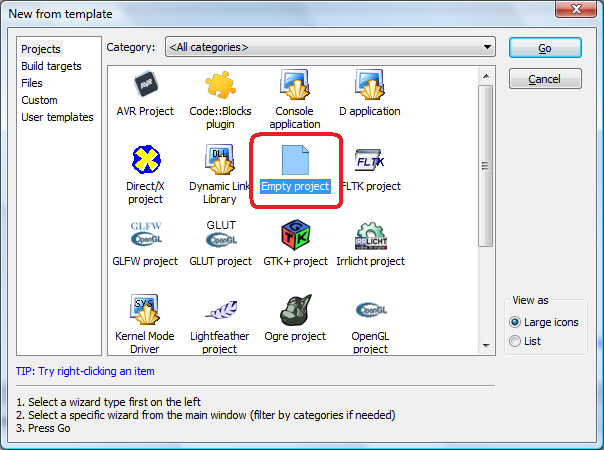
\includegraphics[scale=0.3]{images/cb_new}
\end{center}
\end{frame}

\begin{frame}{Programming in C with Code::Blocks}{Creating project}
\begin{enumerate}
\setcounter{enumi}{2}
  \item Choose  GNU GCC Compiler
  \item Select the next 2 options if you want to create ``debug'' and ``release'' configuration
\end{enumerate}
\begin{center}
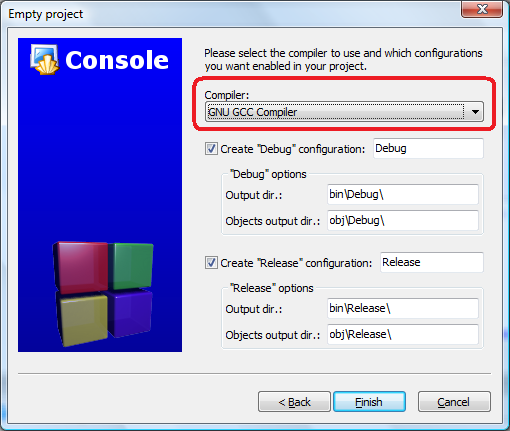
\includegraphics[scale=0.3]{images/cb_compiler}
\end{center}
\end{frame}

\begin{frame}{Adding source file}
\begin{enumerate}
\setcounter{enumi}{4}
  \item Add source file in the project:
  File -> New -> File -> C/C++ Source
  \item Choose C as programming language 
  \item Enter the file name with the full path, and don't forget to check ``Add
  file to active project''
\end{enumerate}
\begin{center}
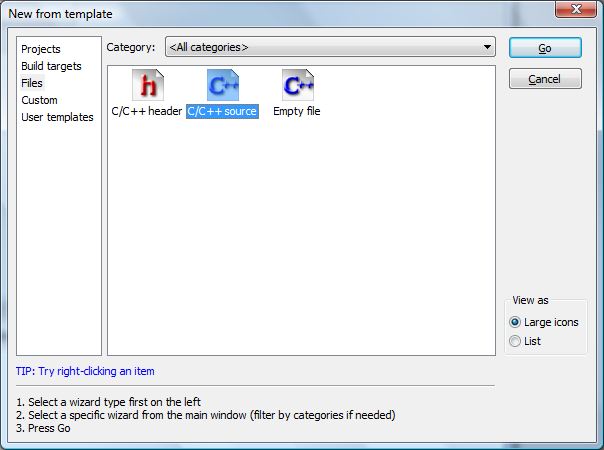
\includegraphics[scale=0.25]{images/cb_source}
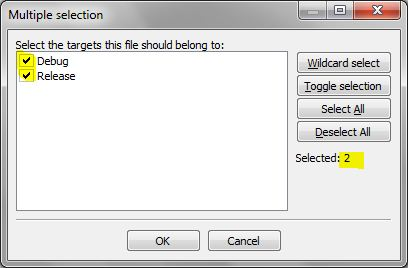
\includegraphics[scale=0.4]{images/cb_include}
\end{center}
\end{frame}

\begin{frame}{Programming}
\begin{itemize}
  \item For each project following options can be checked ``Project Build
  Options.. Compiler Flags''
  \item To build the project press Ctrl + F9
  \item To execute the project press Ctrl + F10
\end{itemize}
\begin{center}
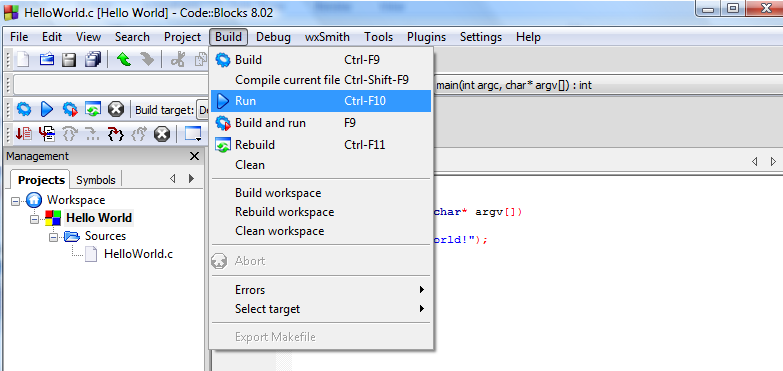
\includegraphics[scale=0.25]{images/cb_run}
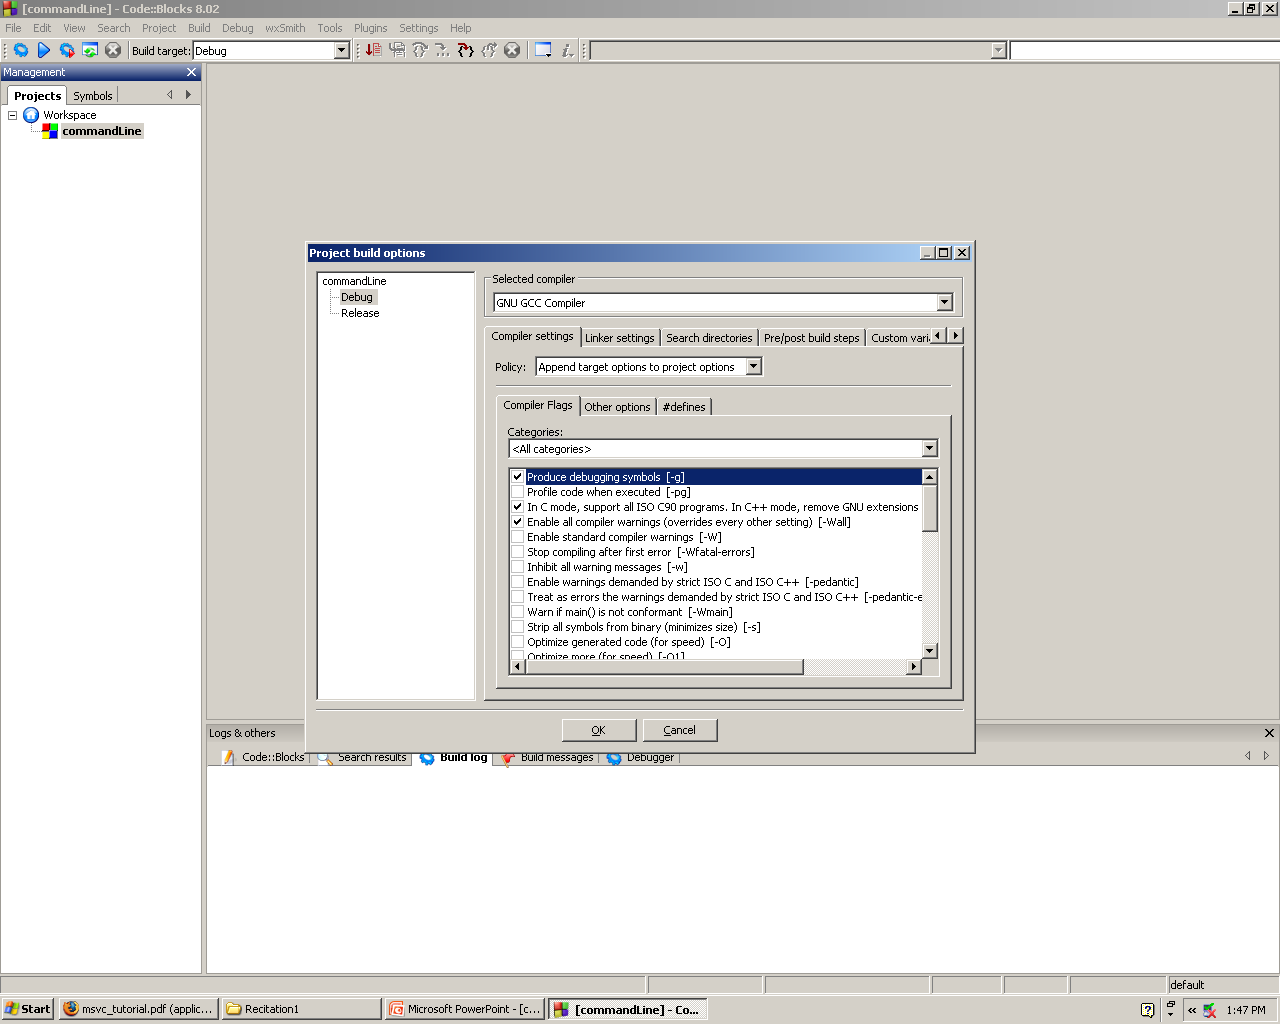
\includegraphics[scale=0.1]{images/cb_flags}
\end{center}
\end{frame}

\begin{frame}{Homework}
\begin{itemize}
  \item In the next section are given some example problems that you should
  try to complete at home
  \item so you can be ready for next excersises
\end{itemize}
\end{frame}

\begin{frame}[fragile]{Problem 1}
Try to create new project with one \texttt{.с} file with the following source
code:
\begin{lstlisting}
#include <stdio.h>

int main() {
    printf("Hello, how are doing?\n");
    return 0;
}
\end{lstlisting}

\end{frame}

\begin{frame}{Problem 1}
\begin{itemize}
  \item Execute the program
\begin{itemize}
  \item What result do you get?
\end{itemize}
  \item If you made some errors during writing the code, try to find,
  correct them and execute again.
  \item Make some errors, intentionally. Execute again!
\begin{itemize}
  \item What's happening now?
\end{itemize}
\end{itemize}
\end{frame}

\begin{frame}[fragile]{Problem 2}
\definecolor{light-gray}{gray}{0.90}
In the text of te program add the following line:
\begin{lstlisting}
#include <stdio.h>
int main() {
    printf("Hello, how are you doing?\n");
    printf("So, you are not much of a talker...\n"); 
    return 0;
}
\end{lstlisting}
What is the result now?
\end{frame}
